\section{Specifying Compiler Correctness}
\label{sec:terminology}

%% The previous section stated Coq theorems in terms of simulations, without giving definitions.
%% Here are the definitions.

\subsection{Abstract Correctness}

CompCert is a compiler.
As a compiler user, CompCert translates my C99 programs to executable files.

\begin{center}
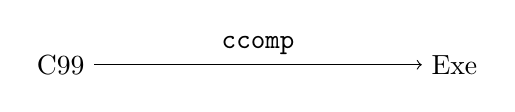
\begin{tikzpicture}
  \node (0) {C99};
  \node (1) [right of=0,xshift=4cm]{Exe};
  \draw[->] (0) -- node[above]{{\tt ccomp}} (1);
\end{tikzpicture}
\end{center}

This translation is correct if the executable performs the same sequence of operations that the source program \emph{should} perform, if I was to interpret it line-by-line.
For instance, the executable for the program on the left should print to the console exactly once and exit cleanly.
The executable for the program on the right should print to the console until I forcibly kill the program.

\hbox{
\begin{lstlisting}
    int main(void) {
      printf("Hello\n");
      return 0;
    }
\end{lstlisting}\hspace{3cm}\begin{lstlisting}
int main(void) {
  while (1) printf("Hello\n");
  return 0;
}
\end{lstlisting}
}

More precisely, a correct compiler will translate the semantics of the source program into equivalent semantics in the target program.
There are generally a few ways to specify this notion of \emph{semantics preservation}.
CompCert uses simulations.


\subsection{Notions of Simulation}

Let $\compil$ be a compiler from source language $\srclang$ to target language $\tgtlang$.
Suppose $\srcprog$ is a program written in language $\srclang$ and $\tgtprog$ is the result of compiling $\srcprog$.
In other words, $\tgtprog = \compil(\srcprog)$.

Suppose the semantics for $S$ imply that $\srcprog$ should begin at state $\srcprog_0$, run for $n$ steps, and halt at the final state $\srcprog_n$.
Also suppose that $\tgtprog$ begins at state $\tgtprog_0$, runs for $m$ steps, and finishes at state $\tgtprog_m$.
Some of the transitions on either side may cause an observable effect, like printing to the screen or closing a file, so we label each edge with a tag $e$ describing the effect (if any).
Our general picture is now:

\begin{center}
\begin{tikzpicture}
  \node (00) {$\srcprog_0$};
  \node (01) [below of=00] {$\srcprog_1$};
  \node (02) [below of=01] {$\vdots$};
  \node (03) [below of=02] {$\srcprog_n$};

  \node (10) [right of=00,xshift=4cm] {$\tgtprog_0$};
  \node (11) [below of=10] {$\tgtprog_1$};
  \node (12) [below of=11] {$\vdots$};
  \node (13) [below of=12] {$\tgtprog_m$};

  %% \draw[->] (00) -- node[above]{$\compil$} (10);

  \draw[->] (00) -- node[left]{$e_{s1}$} (01);
  \draw[->] (01) -- node[left]{$e_{s2}$} (02);
  \draw[->] (02) -- node[left]{$e_{sn}$} (03);

  \draw[->] (10) -- node[right]{$e_{t1}$} (11);
  \draw[->] (11) -- node[right]{$e_{t2}$} (12);
  \draw[->] (12) -- node[right]{$e_{tm}$} (13);
\end{tikzpicture}
\end{center}

Our goal is to prove by simulation that $\srcprog$ and $\tgtprog$ are equal programs based on their transition structure.


\subsubsection{Bisimulation}

A straightforward technique is to demonstrate a \emph{bisimulation} relation between the source and target.
This amounts to giving a relation $\bisim$ such that:
\begin{itemize}
\item $(\srcprog_0, \tgtprog_0) \in \bisim$
\item For all states $\srcprog_i$, $\stepsto{\srcprog_i}{\srcprog_{i+1}}{e_{s(i+1)}}$
      implies that for all target states such that $(\srcprog_i, \tgtprog_j) \in \bisim$, there exists a target state $\tgtprog_{j+1}$ such that $\stepsto{\tgtprog_j}{\tgtprog_{j+1}}{e_{t(j+1)}}$
      and $(\srcprog_{i+1}, \srcprog_{j+1}) \in \bisim$.
      Also, $e_{s(i+1)}$ and $e_{t(j+1)}$ are the same effect.
\item The reverse holds for target transitions:
      For all states $\tgtprog_j$, $\stepsto{\tgtprog_j}{\tgtprog_{j+1}}{e_{t(j+1)}}$
      implies that for all source states such that $(\srcprog_i, \tgtprog_j) \in \bisim$,
      there exists a source state $\srcprog_{i+1}$ such that $\stepsto{\srcprog_i}{\srcprog_{i+1}}{e_{s(i+1)}}$
      and $(\srcprog_{j+1}, \tgtprog_{j+1}) \in \bisim$
      Also, $e_{s(i+1)}$ and $e_{t(j+1)}$ are the same effect.
\end{itemize}

In terms of the picture above, the proof would require $n = m$ and for each $i \in \{0..n\}$, $(\srcprog_i, \tgtprog_i) \in \bisim$.


\subsubsection{Backward Simulation}
Bisimulation is a very strong notion of equivalence, but it definitely shows that $\srcprog$ and $\tgtprog$ are equal, in the sense that every action of the source is matched by an action in the target, and vice-versa.
It is so strong that it disallows basic compiler optimizations: if the source program contains no-op instructions, the compiled version must take the same number of do-nothing transitions.
A \emph{backward simulation} $\backsim$ allows these optimizations.
The requirements are:
\begin{itemize}
\item $(\srcprog_0, \tgtprog_0) \in \backsim$
\item All target transitions are matched by \emph{one or more} source transitions.
      For all states $\tgtprog_j$, $\stepsto{\tgtprog_j}{\tgtprog_{j+1}}{e_{t(j+1)}}$
      implies that for all source states such that $(\srcprog_i, \tgtprog_j) \in \backsim$,
      there exists a source state $\srcprog_{k}$ such that $\stepstoplus{\srcprog_i}{\srcprog_{k}}{e_{sk}}$
      and $(\srcprog_k, \tgtprog_{j+1}) \in \backsim$.
      Also, $e_{sk}$ and $e_{t(j+1)}$ are the same effect.
\end{itemize}
The notation $\longrightarrow^+$ denotes one or more transitions.\footnote{Allowing a sequence of transitions means we need to compose effects. For simplicity, assume that the only way to compose effects is to delete a null effect from the left or right end of a sequence.}
This way, our compiler is free to make $\tgtprog$ a more efficient version of $\srcprog$.


\subsubsection{Forward Simulation}
Another useful notion of simulation is to remove the third bisimulation requirement, but keep the second.
As with backwards simulations, it is useful for \emph{forward simulations} to accept multiple target steps in response to one source step.
\begin{itemize}
\item $(\srcprog_0, \tgtprog_0) \in \fwdsim$
\item For all states $\srcprog_i$, $\stepsto{\srcprog_i}{\srcprog_{i+1}}{e_{s(i+1)}}$
      implies that for all target states such that $(\srcprog_i, \tgtprog_j) \in \fwdsim$,
      there exists a target state $\tgtprog_{k}$ such that $\stepsto{\tgtprog_j}{\tgtprog_{k}}{e_{tk}}$.
      Also, $e_{s(i+1)}$ and $e_{tk}$ are the same effect.
\end{itemize}


\subsubsection{Measured Forward Simulation}
CompCert proves many of its optimizing passes using forward simulations augmented by a well-founded measure.
The general shape of these proofs is to use a measure $<$ on source states to prove a relation $\fwdsim$ such that:
\begin{itemize}
\item Given a source program $\srcprog$ and compiled version $\tgtprog$, we have $(\srcprog, \tgtprog) \in \fwdsim$
\item Whenever the source program takes a step to $\srcprog'$, either:
  \begin{itemize}
  \item The target program takes a step, and the results of each step are related by $\fwdsim$
  \item The target program does \emph{not} step, but $(\srcprog', \tgtprog) \in \fwdsim$ and $\srcprog' < \srcprog$.
  \end{itemize}
\end{itemize}
The last scenario is a \emph{stutter} in the source.
The measure $<$ ensures that we do not stutter forever, but rather make progress at some point.
As an example, $<$ might count the number of no-ops in a program and $\tgtprog$ might be a version of $\srcprog$ with all no-ops removed.
It should be easy to show that all transitions of source and target match, except in the case that the source program performs a no-op.


\subsubsection{Composition}
CompCert's proof of correctness relies on two properties of simulations.
We name and sketch proofs of these simulations, assuming for simplicity that there are no effects and no skipping transitions.
Full proofs are in the CompCert repository.

\textbf{Forward Simulations Compose} [\href{https://github.com/AbsInt/CompCert/blob/master/common/Smallstep.v#L798}{proof}] \quad
 Suppose we have two forward simulations: one from $\srclang$ to $\tgtlang$ and the other from $\tgtlang$ to $\tgtlang'$.
Call these $R_1$ and $R_2$, respectively.
We claim that $R_3 = \{\,(\srcprog_i, \tgtprog'_k) \mid (\srcprog_i, \tgtprog_j) \in R_1 \wedge (\tgtprog_j, \tgtprog'_k) \in R_2\,\}$ is a forward simulation from $\srclang$ to $\tgtlang'$.

First, all initial states of $\srclang$ and $\tgtlang'$ are related by construction: if $\srcprog_0$ is an initial state, then it must be related by $R_1$ to some $\tgtprog_0$ and likewise $R_2$ must relate $\tgtprog_0$ to some initial state $\tgtprog'_0$.
Therefore $R_3$ relates $\srcprog_0$ to $\tgtprog'_0$.
Second, if $\srcprog_i$ steps to $\srcprog_{i'}$ and $(\srcprog_i, \tgtprog_j) \in R_1$ then:
\begin{itemize}
\item There exists a $\tgtprog_{j'}$ such that $\tgtprog_{j} \rightarrow \tgtprog_{j'}$ and $(\srcprog_{i'}, \tgtprog_{j'}) \in R_1$
\item If there is an $\tgtprog'_{k}$ such that $(\tgtprog_j, \tgtprog'_k) \in R_2$ then there exists a $\tgtprog'_{k'}$ such that $\tgtprog'_k \rightarrow \tgtprog'_{k'}$ and $(\tgtprog_{j'}, \tgtprog'_{k'}) \in R_2)$.
\item By construction, $(\srcprog_i, \tgtprog'_k) \in R_3$
\item The state $\tgtprog'_{k'}$ matches the transition from $\srcprog_i$ to $\srcprog_{i'}$.
\end{itemize}

\textbf{Forward Simulations imply Backward Simulations} [\href{https://github.com/AbsInt/CompCert/blob/master/common/Smallstep.v#L1481}{proof}] \quad
 If we have a deterministic target language, then a forward simulation from source to target implies a backward simulation from target to source.
Suppose $(\srcprog_i, \tgtprog_j)$ are related source and target states and furthermore $\tgtprog_j \rightarrow \tgtprog_{j'}$.
We know that $\tgtprog_{j'}$ is unique because the semantics is deterministic.
So it must be true that all transitions out of $\srcprog_i$ match the transition from $\tgtprog_j$\textemdash otherwise, we would contradict our assumed forward simulation.\footnote{I didn't fully understand the Coq proof, but as far as I can tell it is classical. Being classical is not such a big deal because there are finitely many transitions out of each state.}


\subsection{Proving a Compiler}
Let $\simeq$ be one of the above simulations.
A verified compiler $\compil$ guarantees that for all source programs $\srcprog$, if $\compil(\srcprog) = \tgtprog$ then $\srcprog \simeq \tgtprog$.
Note that if the compiler fails to produce a result, we have no $\tgtprog$ and no theorem.
Making sure that a compiler successfully compiles all valid source programs is an important engineering issue~\cite{l-formally}.

One way to verify a compiler is to reason directly about its source code.
This is straightforward, but potentially difficult and less efficient~\cite{b-size} than an unverified compiler.

An alternative is to use an unverified compiler along with a \emph{translation validator} $\valid$, and abort compilation if the validator rejects the compiler's results.
The guarantee would then be: for all source programs $\srcprog$, if $\compil(\srcprog) = \tgtprog$ and $\valid(\tgtprog) = \mathsf{true}$ then $\srcprog \simeq \tgtprog$.
This approach shifts the proof effort to the validator.
If one can show that the validator correctly recongizes valid and invalid results, we have a verified compiler.

As we shall see, CompCert uses both techniques.

%% \subsection{Alternatives: PCC \& Witnesses \& Logical Relations}
%% PCC : don't prove, just attach evidence and the client will check
%% Witnesses : help the validator
%% LR : ???

